\documentclass{standalone}
\usepackage{pgfplots}
\usepackage{fontspec}
\setmainfont{xkcd}

\begin{document}

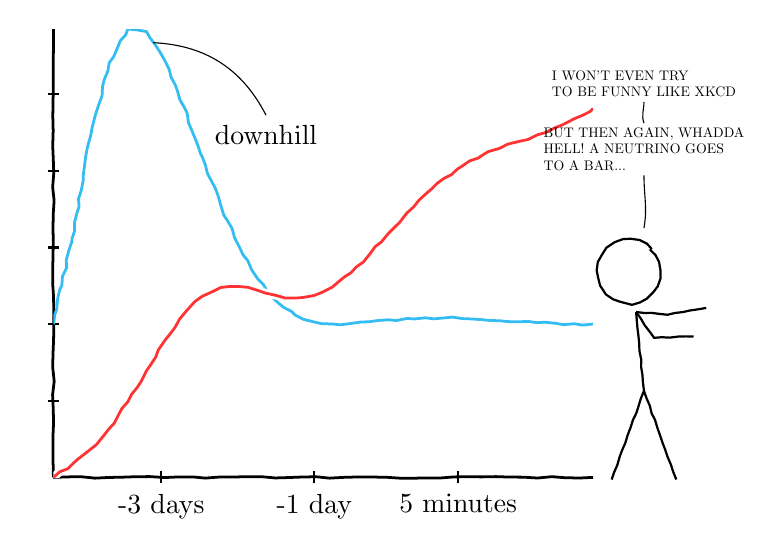
\begin{tikzpicture}[decoration={random steps,segment length=1mm,amplitude=0.2pt}]
	\pgfplotsset{every axis/.append style={line width=1pt}}

	\begin{axis}[%
			axis x line=middle,
			axis y line=middle,
			xtick={1.2, 2.9, 4.5},
			xticklabels={-3 days, -1 day, 5 minutes},
			yticklabels={},
			every inner x axis line/.append style={-},
			every inner y axis line/.append style={-},
			decoration={random steps,segment length=5pt,amplitude=0.3pt},decorate,
			every tick/.style={thick,black,decorate}
		]
		\begin{scope}[decoration={random steps,segment length=3pt,amplitude=0.5pt},decorate]
			\addplot [cyan!80!white, samples=30, domain=0:6] {3+(sin(deg(x))^2)/sqrt(x)*exp(-(x-2))};
			\addplot [white,double=red!80!white, samples=30, domain=0:6,double distance=1.0pt] {0.4*x+2+x^2*sin(deg(x))^2*exp(-x)};
		\end{scope}
	\end{axis}
	\draw (1.2679,5.5206) to[bend left] (2.7,4.6) node[below] {downhill};
	\begin{scope}[shift={(7cm,3cm)},thick]
		\draw[line join=round,decorate] (0.6cm,-0.1cm) arc (45:275:0.4cm) arc (275:410:0.38cm);
		\draw[decorate] (0.4cm,-0.9cm)coordinate (n) -- ++(0.1,-1cm) coordinate (a) -- +(-70:1.2cm) (a) --+(-110:1.2cm);
		\draw[decorate] (n) -- ++(-5:0.4cm) --+(10:0.5cm);
		\draw[decorate] (n) -- ++(-55:0.4cm) --+(2:0.5cm);
		\node[align=left,scale=0.5] (c) at (0.5,2){I WON'T EVEN TRY \\TO BE FUNNY LIKE XKCD};
		\draw[thin] (c) to[in=110,out=-90] ++(0,-0.5cm) node[below,align=left,scale=0.5]
		(d) {BUT THEN AGAIN, WHADDA\\ HELL! A NEUTRINO GOES \\TO A BAR...};
		\draw[thin] (d) to[in=80,out=-90] ++(0,-1cm);
	\end{scope}

\end{tikzpicture}

\end{document}
